\RequirePackage{luatex85}
\documentclass[a4j]{ltjsarticle}
\usepackage{mymacros}
\usepackage{graphicx}
\usepackage[hiragino-pro]{luatexja-preset}
\usepackage{luatexja-ruby}
\usepackage{luatexja-otf}
\DeclareMathAlphabet{\mathrsfs}{U}{rsfso}{m}{n}
\renewcommand{\mathscr}[1]{\mathup{\mathrsfs{#1}}}
\usepackage[super]{nth}
\usepackage[bookmarksnumbered,pdfproducer={LuaLaTeX},%
            luatex,psdextra,pdfusetitle,pdfencoding=auto]{hyperref}
\usepackage[backend=biber,style=math-numeric]{biblatex}
\addbibresource{myreference.bib}
\renewcommand{\emph}[1]{\textsf{\textgt{#1}}}
\newcommand{\leport}{$\lambda$eport}

\usepackage{url}	% required for `\url' (yatex added)
\usepackage{amssymb}	% required for `\mathbb' (yatex added)
\begin{document}
\begin{center}
 {\huge \bfseries \ruby{石}{いし}\ruby{井}{い} \ruby{大海}{ひろみ}}
 \vskip 1em
 筑波大学数理物質科学研究科\\
 数学専攻 博士後期課程\\
 \textsc{E-Mail}: \href{mailto:h-ishii@math.tsukuba.ac.jp}{\nolinkurl{h-ishii@math.tsukuba.ac.jp}}\\
 \textsc{Web Site}: \url{https://konn-san.com}\\
 \textsc{GitHub}: \url{https://github.com/konn}
\end{center}

\section*{基本情報}
\begin{description}
 \item[氏名] 石井 大海(いしい・ひろみ)
 \item[性別] 男
 \item[生年月日] 1992年1月18日
\end{description}

\section*{教育・学位}
\begin{tabular}[t]{@{}p{.2\linewidth}p{.75\linewidth}@{}}
 \begin{minipage}[t]{\linewidth}\emph{博士(理学),予定}\\ 2016年4月〜現在\end{minipage} 
 & 筑波大学数理物質科学研究科数学専攻 博士後期課程\\[2em]
 \begin{minipage}[t]{\linewidth}\emph{修士(理学)}\\ 2016年3月\end{minipage} 
 & \begin{minipage}[t]{\linewidth}
    筑波大学数理物質科学研究科 博士前期課程・修了\\
   \emph{修士論文:} On Regularity Properties of Sets of Reals and Inaccessible Cardinals
   \end{minipage} 
 \\[3em]
 \begin{minipage}[t]{\linewidth}\emph{学士(理学)}\\2014年3月\end{minipage} 
 & 早稲田大学基幹理工学部数学科・卒 \\
\end{tabular}

\section*{職歴・採用歴}
\begin{description}
 \item[2017年4月〜2019年3月]
              日本学術振興会特別研究員 DC2

              研究課題:『実数の集合の性質の集合論的解明と工学的応用』
 \item[2017年4月〜] 筑波大学数学専攻計算機管理オブザーバー
 \item[2014年〜2017年] 筑波大学数学類『計算機演習』ティーチング・アシスタント
 \item[2014年4月] Google Summer of Code 2014採択

            題目:『Haskellによる効率的なGr\"{o}bner基底計算とそのための疎行列対角化アルゴリズムの実装』
 \item[2014年4月〜2017年3月] 筑波大学数学専攻計算機管理アルバイト(www-admin)
 \item[2010年10月〜2014年3月] 株式会社Preferred Infrastructureアルバイト
 \item[2010年8月〜9月] 株式会社Preferred Infrastructureインターン生
\end{description}

\section*{賞罰・特記事項}
\begin{itemize}
 \item 日本学術振興会特別研究員DC2,(2017年〜2019年)
 \item 第十四回茗渓会賞(2016年)
 \item 2013年度早稲田大学基幹理工学部長賞最優秀賞(第一回)
 \item 2013年度早稲田大学基幹理工学部卒業生総代
 \item Web数式処理ライブラリ\href{https://github.com/Khan/KaTeX}{KaTeX}コミッタ
 \item Haskell製Webフレームワーク\href{https://www.yesodweb.com}{Yesod}コミッタ
\end{itemize}

\subsection*{出版前レビュー担当書}
\begin{itemize}
 \item 『すごいHaskell楽しく学ぼう!』,M. Lipova\v{c}a=著, 田中英行・村主崇行=共訳,オーム社,2012年,\textsf{ISBN}: \texttt{978-4274068850}.
 \item 『型システム入門──プログラミング言語と型の理論──』,B. C. Pierce=著,住井英二郎=監訳,遠藤侑介・酒井政裕・今井敬吾・黒木裕介・今井宜洋・才川隆文・今井健男=共訳,オーム社,2013年,\textsf{ISBN}: \texttt{978-4274069116}.
 \item 『Haskellによる並列・並行プログラミング』,S. Marlow=著,山下伸夫・山本和彦・田中英行=共訳,オライリー・ジャパン,2-14年,\textsf{ISBN}: \texttt{978-4873116891}.
 \item ほか1冊
\end{itemize}

\section*{研究業績}
\begin{refsection}
 \subsection*{研究分野概説}
主な研究分野は\emph{数理論理学},とくに\emph{公理的集合論}と呼ばれる分野である.
公理的集合論は主に実数の集合や,一般の無限について研究する数学の一分野である.
集合論においてモデルの構成に用いられる\emph{強制法}は,理論計算機科学における$\lambda$-計算のモデルである\emph{Scott領域}と深い関係があり,Krivineの実現可能性モデル\cite{Krivine:2011jk,Krivine:2012hl,Krivine:2016if}として結実した.

私の興味分野はこうした集合論のモデルの構成法一般であり,そうしたモデルにおける実数の振る舞いである.
現在メインで取り組んでいる物は飽和イデアルという物から得られる集合論のモデルである.
一方で,上記の実現可能性モデルのような,計算論的背景を持つモデルにおける実数の集合性質を,実際に計算機上で実現することは出来るか?という問題意識も持っており,これが現在採用中の日本学術振興会特別研究員の研究課題の一つにもなっている.
 \printbibliography[title=参考文献,heading=subbibliography]
\end{refsection}

\subsection*{査読付き学会発表}
\noindent
March 2016, \emph{Freer Monads, More Extensible Effects}. Programming and Programming Language Workshop (PPL) 2016, Okayama-prefecture, Japan.

\subsection*{査読無し学会発表}
\noindent
November 2017, \emph{Reflection Principle and construction of saturated ideals on $\Pow_{\omega_1} \lambda$}. Workshop on Iterated Forcing Theory and Cardinal Invariants, Kyoto-prefecture, Japan.

\begin{refsection}
 \nocite{ISHII:2016sf,Kiselyov:2015xy}
 \printbibliography[title=論文,heading=subbibliography]

 上記の\cite{Kiselyov:2015xy}は関数型言語において複数の副作用を合成する手法を提案したものであり,Oleg Kiselyov氏との共同研究である.
\end{refsection}

\section*{スキルセットと開発実績}
\begin{refsection}
主に関数型プログラミング言語Haskellを用いた汎用プログラムの開発を得意とする.
特に,Haskellの特性を活かした並行・分散処理の記述や,型システムの機能を応用した安全なソフトウェアの開発に大きな関心がある.
得意とする開発スキルセットを以下に挙げる:

\begin{itemize}
 \item \emph{型システム}や\emph{性質ベーステスト}などの\emph{形式手法}を用いた\emph{信頼性の高いプログラム}の開発.
 \begin{itemize}
  \item 定理証明系Agda \cite{Agda:2018zh}を用いた(構成的)数学の形式化経験もあり.
 \end{itemize}
 \item \emph{数学的なアルゴリズム},特に計算機代数の効率的な実装.
 \item \emph{高度な分散・並行処理}を用いたプログラムの開発.
 \item Haskellを用いた\emph{実践的なWebアプリケーション}の開発.
 \item パーザや構文木の操作を通じたメタプログラミングや文書の生成.
\end{itemize}

開発経験のある言語は,頻度順で次の通りである:
\begin{itemize}
 \item Haskell
 \item JavaScript, CoffeeScript
 \item Ruby (〜1.9), Objective-C
 \item Agda
\end{itemize}

また,筑波大学の数学類\footnote{通常の大学で学部の数学科に相当する.}の学生を対象とした演習『計算機演習』では,2014年度よりHaskellを学生に教えているが,この講義の立ち上げ・運営に参画し,ティーチング・アシスタントとしてレポート採点システムの開発や授業計画案の提言などを行っている.
また,後述する計算機代数ライブラリを用いた,数学類生の卒業研究にティーチング・アシスタントとして参加し,Haskellによる開発手法を生徒らに教育した.
こうした活動を通して,個人としての開発能力だけでなく,プログラミング教育のスキルも日々磨いている.

以下,過去に従事した開発事例を幾つか紹介する.

\subsection*{レポート自動採点システム\leport}
 上述した「計算機演習」において,生徒の提出したレポート(Haskellプログラム)を自動採点するためのツールである.
 演習のティーティング・アシスタントにはそこまでHaskellに習熟していない担当者もおり,また単なる目視による採点では見落としがあり得る.
 そこで,関数型プログラミングにおける\emph{性質ベーステスト}(\emph{Proeprty-based Testing})の方法論を応用し,レポートの答案の形式仕様を与え,生徒の答案がその仕様を満たすかを自動でチェックし,結果を報告する\emph{自動採点システム\leport{}}を構築した.
 この大まかな構造を図\ref{fig:leport-structure}に示した.

 \begin{figure}[htbp]
 \centering
 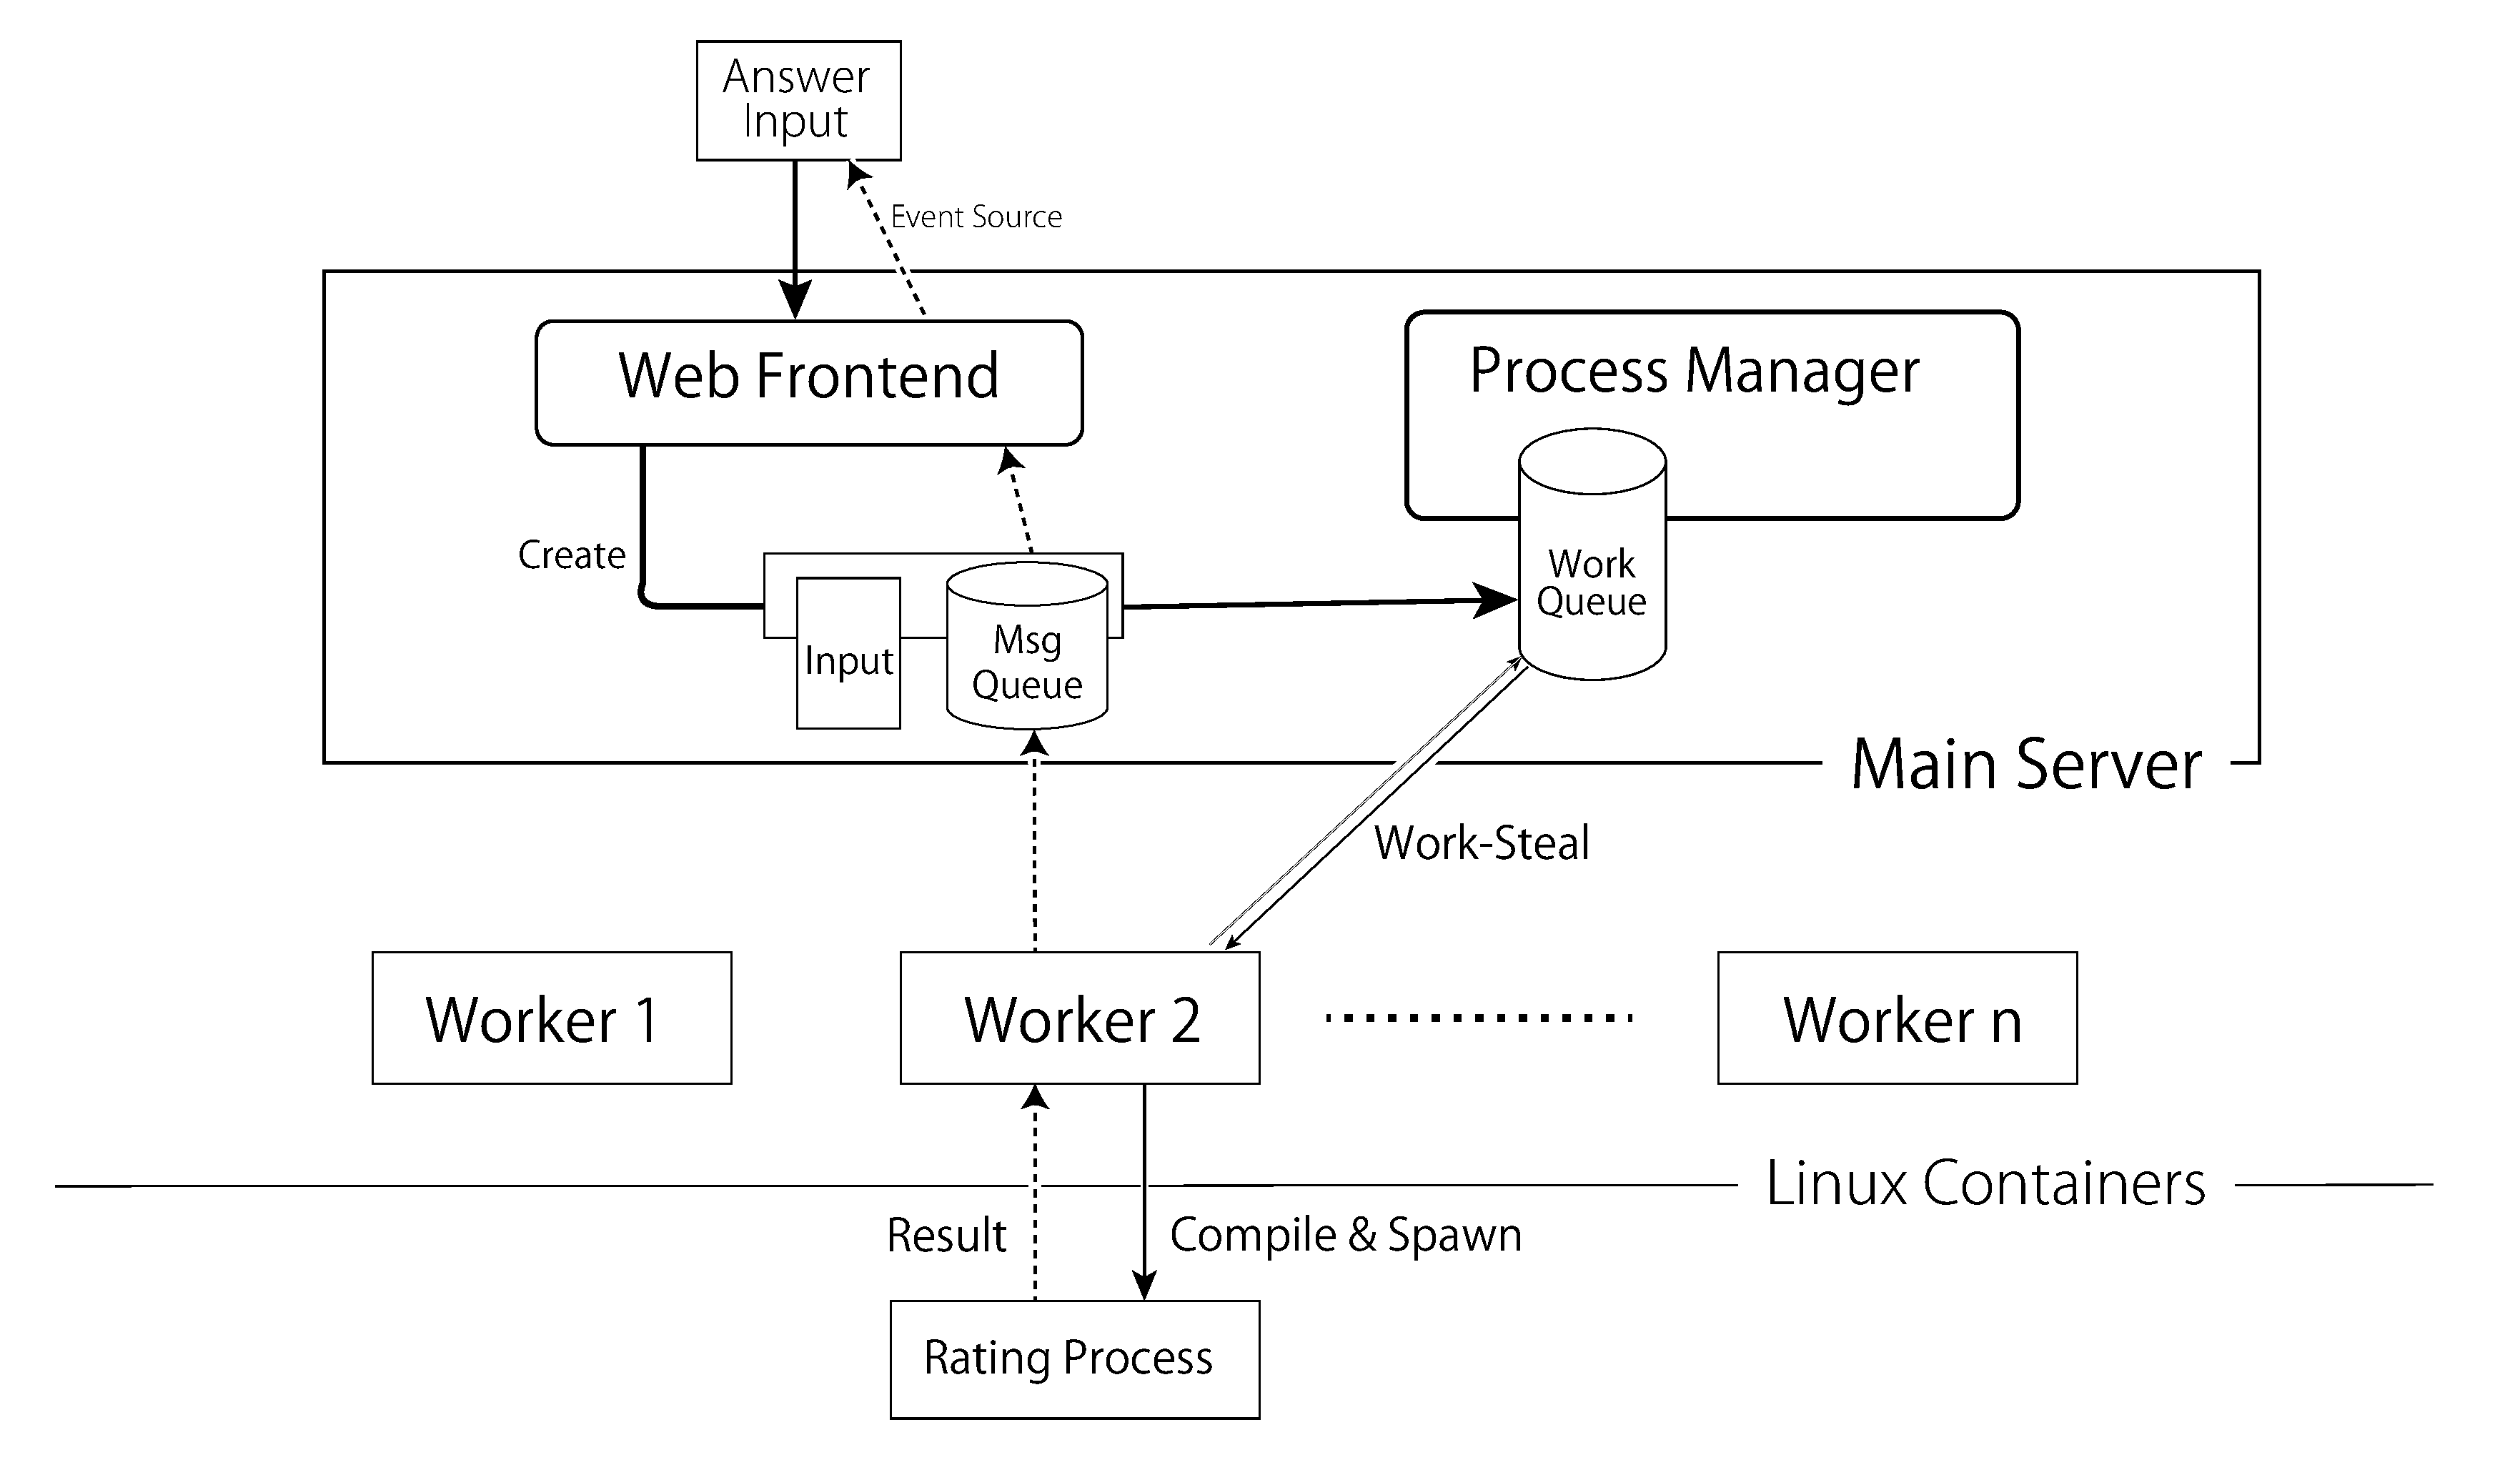
\includegraphics[width=.8\paperwidth]{cv/leport-structure.pdf}
 \caption{\leport{}の構造}\label{fig:leport-structure}
 \end{figure}

 \leport{}を設計するに当たっては,その性質上以下のような要請があった:

 \begin{description}
 \item[プライバシー] 生徒の答案を扱うため,HTTPS上で通信が行われる必要性がある.
 \item[並行性] 複数人のティーティング・アシスタントが同時に採点を行うため,一度に複数の採点プロセスを走らせる必要性がある.
 \item[安全性] 生徒の答案を入力するため,任意のコードが実行される畏れや,無限ループに陥りマシンリソースが食い潰される可能性がある.
 \item[リアルタイム性] 採点結果はなるべく早く,各小問ごとに結果がわかるとよい.
 \end{description}

 以上の要請を満たすために,本システムでは以下の技術を用いている:

 \begin{description}
 \item[Let's Encrypt] \emph{セキュア}な通信のために,Let's Encrypt \cite{letsencrypt:2017si}の発行する無料の証明書を利用し,通信を暗号化した.
 \item[Cloud Haskell] \emph{並行性}を実現するため,Haskellによる分散コンピューティングライブラリである\emph{Cloud Haskell} \cite{Well-Typed:2017wq}を採用した.
            図\ref{fig:leport-structure}に示した通り,問題の入力を受け付けたメイン・サーバのキューから別途ワーカ・プロセスが読み出すWork-Steal方式により,効率的な分散処理を実現した.
  \item[Softoware Transactional Memory (STM)]
   一方,ワークキューへの登録や採点プロセスからのログのリレーなどメインサーバ内で並行処理をスレッド安全に実現するために,GHCの提供する\emph{Software Transactional Memory}の機構を利用した.
   特に並行処理対応のキューを用いることで,ロジックを宣言的・受動的に書く事が出来,簡潔な記述が可能になった.
 \item[Linux Containers]
  Linux Containers~\cite{lxc:2017sy}技術を利用することで,サーバ上に隔離されたコンテナ環境を作り出し,生徒の答案をコンテナ内部でコンパイル・実行することで,\emph{安全性}を確保した.
  Linux ContainersにはCPUやメモリの占有率を設定・制御する機構があるため,必要以上のリソースが採点プロセスによって食い潰される事も防ぐことができる.

  実際にはLinux Containersのコンテナマネージャである\emph{LXD}インターフェースを介してコンテナの操作を行った.
  これは,HaskellのLXCバインディングでは使えない機能も多いのに対して,HTTPを介したREST APIを提供しているLXDの方が柔軟性や機能面で優位であったためである.
  LXDはWebSocketを経由したプロセス通信の枠組みを用意しており,これをリレーすることで\emph{リアルタイム性}も実現した.
  \item[EventSource]
  採点プロセスとWebフロントエンドの\emph{リアルタイム}通信には\emph{EventSource}を用いた.
  類似技術のWebSocketに較べて,プロトコルやエンドポイントを切り替える必要がなく,通信はサーバからクライアントへの一方通行で良いため,EventSourceを採用した.
  \item[QuickCheck]
  性質ベーステストライブラリであるQuickCheck~\cite{Claessen:2018rx}を用いてレポート問題の形式仕様を記述し,ランダムテストを走らせることで答案の正誤を判定している.
 \end{description}

\subsection*{Haskell上の計算機代数システム\texttt{computational-algebra}}
 \noindent
 \textsc{Web Site}: \url{https://konn.github.io/computational-algebra}

 関数型言語Haskellの旗艦処理系であるGlasgow Haskell Compiler(以下,GHC)が提供するリッチな型システムを活かし,高度な数学的計算を型安全に行えるようゼロから設計・実装した.
 具体的には,型システムや形式手法を応用することで以下の長所を実現した:
 \begin{description}
  \item[型安全] 係数体や変数の数,順番などを型で表すことで,異なる多項式環の元を誤って足してしまう,といった誤操作を防止する.
  \item[高い表現力] 型レベル自然数を用いることで,$\mathbb{F}_5$や$\mathbb{F}_{25}$といった有限体を扱うことが出来る.
  \item[直感的] 上の設計により$\Q[x, y, z]$と$\Q[x,z,y, w]$は型上区別されるが,これらの間の埋め込み写像を型情報だけから自動的に計算出来る.
             また,多項式それ自体も本来の数式で書くのと近い形で\verb|#x ^ 2 + #z * #x - 2|のように書くことが出来る.
  \item[正当性の保証] 
     前述の性質ベーステストライブラリQuickCheck \cite{Claessen:2018rx}を用いてアルゴリズムの正当性を静的に検証し,ライブラリの品質を保っている.
 \end{description}

 上述の\emph{Google Summer of Code 2014}においては,高速なGr\"{o}bner基底計算アルゴリズムとして知られる$F_4$ \cite{Faugere:1999}および$F_5$ \cite{Faugere:2002:NEA:780506.780516}アルゴリズムの実装を試み,複数の行列ライブラリを統一的に扱うための枠組みや,代数計算向けのライブラリの整備などを進めた.
 その他にも,有理係数多項式の因数分解や,代数的数の計算機能なども実装されている.

 特に,型安全性を最大限実現するために,GHCの型レベル自然数機能を強化する\texttt{type-natural} \cite{type-natural}パッケージや,コンパイル時にPresburger算術ソルバによって型レベル自然数の扱いを改善するコンパイラプラグイン・\texttt{ghc-typelits-presburger} \cite{ISHII:2017nq}を開発した.
 それらを用い,リストや配列,ベクトルなど任意のシーケンシャルなデータ型に対して,そこから固定長のコンテナ型を創り出せる\texttt{sized} \cite{ISHII:2017wk}パッケージも合わせて開発した.

 本ライブラリは,筑波大学数学類の卒業研究や,エクアドル大学のヤチャイ技術大学の研究プロジェクト等でも用いられている.

\subsection*{その他の開発活動}
\begin{itemize}
 \item Web上で高速かつ高品質な数式描画を可能とする\emph{KaTeX}~\cite{KhanAcademy:2018ol}に幾つかのコマンド・環境を実装し,コミッタ権限を得た.
       これまで本格的なJavaScript開発はしていなかったが,\texttt{npm}や\texttt{browserify},\texttt{flow}などを用いたワークフローには半日程度でキャッチアップ出来た.
 \item 2014年3月までのPreferred Infrastructure社におけるバイトでは,Haskellを用いた汎用パーザ生成器やTwitterクローラの開発などに従事した.
 \item HaskellのWebフレームワーク\href{https://www.yesodweb.com}{Yesod}のOAuth認証ライブラリの開発(現在は引退).
 \item 個人サイト \href{https://konn-san.com}{\nolinkurl{konn-san.com}}のサーバはレンタルVPS上で走らせている.
       当該サイトのコンテンツは静的サイトジェネレータHakyll \cite{Jeugt:2018pc}によって生成されているが,\LaTeX{}のソースからHTMLとPDFを同時に生成したいという個人的な要求から,\LaTeX{}とHTMLの間の構文変換器を自前で実装している.
 \item その他の開発プロジェクトは,GitHub上(\url{https://github.com/konn})にて見ることが出来る.
\end{itemize}

\printbibliography[title=参考文献,heading=subbibliography]
\end{refsection}
\end{document}
